%% 
%% Copyright 2007, 2008, 2009 Elsevier Ltd
%% 
%% This file is part of the 'Elsarticle Bundle'.
%% ---------------------------------------------
%% 
%% It may be distributed under the conditions of the LaTeX Project Public
%% License, either version 1.2 of this license or (at your option) any
%% later version.  The latest version of this license is in
%%    http://www.latex-project.org/lppl.txt
%% and version 1.2 or later is part of all distributions of LaTeX
%% version 1999/12/01 or later.
%% 
%% The list of all files belonging to the 'Elsarticle Bundle' is
%% given in the file `manifest.txt'.
%% 

%% Template article for Elsevier's document class `elsarticle'
%% with numbered style bibliographic references
%% SP 2008/03/01

\documentclass[preprint,12pt]{elsarticle}
\usepackage{pdflscape}
\usepackage{comment}
\usepackage{amsmath}
\usepackage{enumerate}
\usepackage{graphics}
\usepackage{graphicx}
\usepackage{hyperref}
\usepackage{array}
\usepackage{booktabs}
\usepackage{multirow}
\usepackage{color}


%% Use the option review to obtain double line spacing
%% \documentclass[authoryear,preprint,review,12pt]{elsarticle}

%% Use the options 1p,twocolumn; 3p; 3p,twocolumn; 5p; or 5p,twocolumn
%% for a journal layout:
%% \documentclass[final,1p,times]{elsarticle}
%% \documentclass[final,1p,times,twocolumn]{elsarticle}
%% \documentclass[final,3p,times]{elsarticle}
%% \documentclass[final,3p,times,twocolumn]{elsarticle}
%% \documentclass[final,5p,times]{elsarticle}
%% \documentclass[final,5p,times,twocolumn]{elsarticle}

%% For including figures, graphicx.sty has been loaded in
%% elsarticle.cls. If you prefer to use the old commands
%% please give \usepackage{epsfig}

%% The amssymb package provides various useful mathematical symbols
\usepackage{amssymb}
%% The amsthm package provides extended theorem environments
%% \usepackage{amsthm}

%% The lineno packages adds line numbers. Start line numbering with
%% \begin{linenumbers}, end it with \end{linenumbers}. Or switch it on
%% for the whole article with \linenumbers.
%% \usepackage{lineno}

\journal{Swarm and Evolutionary Computation}
\bibliographystyle{elsarticle-num}

\begin{document}

\begin{frontmatter}

%% Title, authors and addresses

%% use the tnoteref command within \title for footnotes;
%% use the tnotetext command for theassociated footnote;
%% use the fnref command within \author or \address for footnotes;
%% use the fntext command for theassociated footnote;
%% use the corref command within \author for corresponding author footnotes;
%% use the cortext command for theassociated footnote;
%% use the ead command for the email address,
%% and the form \ead[url] for the home page:
%% \title{Title\tnoteref{label1}}
%% \tnotetext[label1]{}
%% \author{Name\corref{cor1}\fnref{label2}}
%% \ead{email address}
%% \ead[url]{home page}
%% \fntext[label2]{}
%% \cortext[cor1]{}
%% \address{Address\fnref{label3}}
%% \fntext[label3]{}

\title{Penguins Search Optimisation Algorithm for Association Rules Mining}

%% use optional labels to link authors explicitly to addresses:
%% \author[label1,label2]{}
%% \address[label1]{}
%% \address[label2]{}

\author[a,b]{Youcef Gheraibia\corref{cor1}}
\ead{Y.Gheraibia@hull.ac.uk}
\author[a]{Sohag Kabir}
\author[c]{Abdelouahab Moussaoui}
\author[d]{Youcef Djenouri}
\author[e]{Peng Yeng Yin}
\author[b]{Smaine Mazouzi}

\address[a]{Department of Computer Science, University of Hull, Hull HU6 7RX, UK}

\address[b]{ Badji Mokhtar-Annaba University, P.O. Box 12, 23000 Annaba, Algeria}

\address[c]{Laboratoire de Recherche en Informatique Appliquée (LRIA), Computer Science Department, University of Sétif, 19000, Algeria}

\address[d]{DTISI, CERIST Research Center, Algiers, Algeria}

\address[e]{Department of Information Management, National Chi Nan University, Taiwan}

\cortext[cor1]{Corresponding author. Tel.: +44-7479-560709 ;}

\begin{abstract}

Association Rules Mining (ARM) is one of the most popular and well-known approaches for the decision-making process. All existing ARM algorithms generate a very large number of association rules with high amount of overlapping. To deal with this issue, we propose a new ARM approach (Pe-ARM) based on penguins search optimisation algorithm (PeSOA). Moreover, a new method of overlapping measure is used in the Pe-ARM to evaluate the amount of overlapping among the generated rules. %Indeed, before the evaluation of the rules, each penguin calculates the amount of overlapping between its rule and all accepted rules. Then, the given rule is rejected without fitness evaluation if at least the amount of overlapping for this rule and one rule from the set of accepted rule is greater than the maximum accepted overlap. 
The proposed approach ensures a good diversification over the whole solution space by utilising the multi-groups behaviour of penguins. Furthermore, the search process is based on the oxygen reserve of each penguin, which helps to accelerate the search process. To demonstrate the effectiveness of the proposed approach, several experiments have been carried out on different datasets and specifically on the biological ones. The results reveal that the proposed approach outperforms different well-known ARM algorithms in both execution time and solution quality. 
\end{abstract}

\begin{keyword}
Association Rule Mining; Penguin Search Optimisation Algorithm; Overlap measure; Biological Data-set; ARM.
%% keywords here, in the form: keyword \sep keyword

%% PACS codes here, in the form: \PACS code \sep code

%% MSC codes here, in the form: \MSC code \sep code
%% or \MSC[2008] code \sep code (2000 is the default)

\end{keyword}

\end{frontmatter}

%% \linenumbers

%% main text
\section{Introduction}
 Association Rules Mining is one of the most challenging and important tasks in data mining~\cite{1}. 
 ARM problem was first introduced by Agrawal and Shafer in~\cite{2} and can be formalised as :
 Let $I=\left\{i_{1},i_{2},i_{3}....i_{n}\right\}$ be a set of items and $T =\left\{t_{1},t_{2},t_{3}....t_{m}\right\}$ be a set of transactions, 
 an association rule is an implication of the form 
 $X \rightarrow Y$ such as $X \subseteq  I$, $Y \subseteq I$, and $X \cap Y = \phi$. 
The sets of items X and Y are called antecedent (left-hand-side or \textit{LHS}) and consequent (right-hand-side or \textit{RHS}) of the given rule 
respectively. The ARM problem consists of extracting among the transactional database $T$, 
all pertinent rules respecting minimum support and minimum confidence constraints. Association rules are the core of many applications like data warehousing for indexing problem~\cite{3},
information retrieval for request processing and educational data mining for improving education system~\cite{4}. Describing hidden patterns 
and different dependencies between the set of data has the potential to efficiently improve
the problem solving process. In the literature, ARM algorithms are divided into two main categories: exact approaches and 
meta-heuristics based approaches. The exact approaches such as Apriori~\cite{5}, FPGrowth~\cite{6}, DIC~\cite{7}, DHP~\cite{8} and Eclat~\cite{9} aim at extracting all possible association rules. However, these algorithms are high time and space consuming when dealing with very large databases with many items and transactions. 
To reduce the computation time of such algorithms, a second category, metaheuristics-based approaches have been proposed. Examples of such approaches include ARMGA~\cite{10} and G3PARM~\cite{11} for evolutionary algorithms, PSO-ARM~\cite{12}, $ACO_R$~\cite{13} and BSO-ARM~\cite{14} 
for swarm intelligence. These algorithms have the potential to give only a subset of all relevant rules. Therefore, two challenges can be derived, the computation time of exact algorithms by exploring all rules space in one hand and the quality of the extracted rules using meta-heuristics based approaches by taking into account the similar rules in the other hand. \\
The penguins search optimisation algorithm (PeSOA) \cite{15} is a recent nature inspired approach based on the collaborative hunting strategies of penguins. The penguins synchronise their dives to reduce the expenditure of energy in the hunting process. This strategy is used in the algorithm to help converging quickly towards an optimal solution. The diversification strategy of the penguins search algorithm allows penguins to explore  the whole solution space efficiently. The search process of penguins is based on the reserve of oxygen which allows penguins to decide whether to accelerate or decelerate while exploring the search space and also to decide whether to search or not in a given region. This has motivated the use of the PeSOA for the association rules mining problem to facilitate efficient exploration of the solution space. We incorporate a new measure to the main process of the penguins search to compute the amount of overlapping between rules to help penguins search process to generate only the non redundant rule with low amount of overlapping among them. \\
In this paper, a new algorithm called Pe-ARM (penguins search optimisation algorithm for association rules mining) is proposed  to find a set of consistent rules with superior quality and a low amount of overlapping among the rules. These set of rules must cover the maximum number of transaction in the database.\\
The remainder of the paper is organised as follows: In the next section, relevant works on association rule mining with diverse applications are presented. 
Then, the penguins search optimisation algorithm is introduced in Section 3, 
followed by the proposed Pe-ARM approach   in section 4. 
The experimental results with both standard and biological data sets are reported in Section 5. 
Conclusion and future perspectives of the the present work are provided in Section 6.

\section{Related Works}
ARM approaches can be divided into two main categories, exact and meta-heuristic based methods.
This section reports some existing ARM approaches from both categories.

\subsection{ARM with exact methods}
The well known ARM exact algorithms are Apriori \cite{5}, AIS (Agrawal, Imielinski, Swami) \cite{1}, 
Eclat \cite{9} and FP-Growth \cite{6}. 
The Apriori algorithm is the most used exact algorithm for association rule mining, starts by finding all item sets that satisfy minimum support 
(frequent item sets) also called large item sets. After that Apriori uses these frequent item sets to generate association rules. 
AIS is the first proposed algorithm for mining association rules. The main drawbacks of this algorithm are that it requires multiple scanning 
of database, i.e., it is time consuming and requires more storage space. FP-growth uses FP-tree structure to compress the database, where 
a divide-and-conquer strategy is performed to decompose the mining tasks and the database as well. When dealing with large transactional database, 
these algorithms become high time and memory consuming. Thereafter, different approaches have 
been proposed to ameliorate the exact methods such as reducing the number of passes over the database, sampling the database, using parallelism, and adding constraints on the structure of rules.

\subsection{ARM with meta-heuristics}
Meta-heuristics have been used to reduce the run time of the existing ARM algorithms. Genetic algorithm is the first evolutionary algorithm used to solve the ARM problem, such as GENAR \cite{16}, GAR \cite{17}. 
Those two methods used the standard version of the genetic algorithm with poor representation of the solutions. Afterward, several methods 
for improving genetic algorithm for association rule mining have been proposed to ameliorate genetic operators and the 
representation of the solutions, such as ARMGA \cite{10}. Two major differences between the classical GENAR and ARMGA are the mutation and crossover methods. Often a hybrid method is used to reduce cost, as well as to improve the original methods. A novel hybrid genetic based algorithm called PQGMA has been applied for association rules mining with the use of simulated annealing for the mutation and the crossover operations respectively.
Quantum computing based method \cite{18} uses an adaptive mutation rate, and provides a diversified population.
G3APRM \cite{11} is a new method for association rule mining  with the use of  genetic programming based on the 
Grammar Guided Genetic Programming to avoid invalid individuals found by genetic programming process. In \cite{19}, 
the authors reviewed all association rule mining algorithms based on genetic algorithm and its hybridisation.

Other methods based on swarm intelligence have been designed for ARM problem. 
Particle swarm optimisation algorithm has been applied for association rule mining \cite{12}, 
in this algorithm particle moves randomly on different neighbourhood and optimise the selection process with the best neighbour. 
The main difference between this method and the AGA is the use of neighbourhood points to improve the search intensification strategy. 
Other swarm intelligence algorithms have also been applied for ARM problem. Firstly, an Ant colony optimisation \cite{20} was employed in health application 
to deal with the health insurance database. ARMBGSA \cite{21} is an association rule mining algorithm based on Newton law of universal gravitation namely 
a gravitational emulation local search algorithm, which is a nature inspired optimisation algorithm. Each rule is modelled as a mass, all the masses attract each other using the law of motion. Each iteration is based on the 
previous one, and take only the k-heaviest masses in order to influence the new masses. The algorithm generates few rules because 
the search space is reduced at each iteration. 
Authors on \cite{22} proposed a new hybrid algorithm called (HBSO-TS) for association rule mining based on hybrid method based on 
Bees Swarm Optimisation (BSO) and Tabu Search (TS). BSO is used to explore the search space so that it can cover most of its neighbours.
 
\subsection{ARM applications for genomic}
Algorithms for Association Rule Mining have been extensively developed in market basket analysis, further studies concerning  biological data sets are already available.
 In \cite{23}, the authors apply association rule mining process for genomic. 
 Ant based Association Rule Mining (Ant-ARM) is employed to discover classification of rules for one particular class only, each ant is used to construct one  Classification Association Rule and change one item set at a time. An improved method for integrated analysis of gene expression has been 
 proposed using additional data \cite{24}. Temporal association rules have been used to represent dependencies between the different factors 
 on gene regulatory network \cite{25}. Recent works of biological data analysis based on association rules mining are reviewed in \cite{26}.

\section{Penguins Search Optimisation Algorithm }

Penguin search optimisation algorithm (PeSOA) is a new swarm based meta-heuristic algorithm which was proposed in \cite{15}. The dietary behaviour of penguins may be explained by the economic reasoning: it comes to a profitable food search activity when the gain of energy is greater than the expenditure required to obtain this gain. Penguins, behaving along the line of foraging predators, must extract information about the time and cost to get food and the energy content of prey in order to choose the course for making their next dive.
 PeSOA is inspired by the penguin's hunting behaviour and it generally works as follows:
  
The population of penguins locates initial position (solution space), then the population is divided into a set of groups, and each group is assigned to a region in the whole solution space. Each penguin then dives and swims under the water for hunting fish while consuming its oxygen reserve. Different forms of communication between penguins are occasionally taken place and the quantities of eaten fish increase. The process is repeated until the specified amount of fish is obtained or the maximum number of iterations is reached. The authors of \cite{15} have shown that the PeSOA outruns genetic algorithms and particle swarm optimisation in obtaining better values for benchmark optimisation functions. 
After a number of dives, the penguin returns to surface and share with its group affiliates the position and quantity of the food found. So the local best of each group continuously
 improves as more members report the food sources. After an entire cycle of the intra-group communication of all the penguin groups, the penguins might migrate to other group's habitat according to the probability of nurture existence of each group in terms of the quantity of food found by all its members.
The oxygen reserve depends on both the gain of the food source and the swimming duration the penguin endures. If the energy gain is positive, the longer the penguin stays under the water, the more quantities of food it catches and thus becomes healthier. Otherwise, the longer the swimming duration, the more oxygen the penguin consumes. Hence, the oxygen reserve is updated according to the amelioration of the objective function. The oxygen reserve increases if the new solution is better than the previous one, and the oxygen reserve decreases in the other case.

\section{Pe-ARM: PeSOA for association rules mining}
\subsection{Encoding}
There are two well known association \textbf{reference needed} rule presentation, binary encoding and
integer encoding. In binary encoding, each solution is represented
by a vector $S$ of $n$ elements where $n$ is the number of items.
The $i^{th}$ element of a given solution $S$ is set to $1$ if the
item $i$ is in the rule and $0$ otherwise. However, in integer
encoding, the solution is represented by a vector $S$ of $k+1$
elements where $k$ is the size of the rule. The first element is
the separator index between antecedent and consequent parts of the
solution. For all others elements $i$ in $S$, if $S[i] = j$ then
the item $j$ appears in the $i^{th}$ position of the rule. In
Pe-ARM, both representations are combined to make the
penguins operations and the fitness computing process easier. Indeed, three
values $(0,1,2)$ are used for interpreting the presence of a given
item in the rule. The value $0$ means that the item is absent in
the rule. The value $1$ means that the item is present in the
antecedent part of the rule. The value $2$ means that the item
participates in the consequent part
of the rule. More formally, we have :
\begin{enumerate}
    \item $S[i] = 0$ if the item $i$ is not in the solution $S$.
    \item $S[i] = 1$ if the item $i$ belongs to the antecedent part of the solution $S$.
    \item $S[i] = 2$ if the item $i$ belongs to the consequent part of the solution $S$.
\end{enumerate}
This representation allows to separate the antecedent part and the
consequent part where each single position of a given solution has
the full interpretable information. Moreover, such representation
is flexible and helps us on the calculation of the overlap
measure.\\
\textbf{Example:} Let's $I=\{i_1, i_2,..., i_{10}\}$ be a set of items.
The solution $S_1=\{0, 0, 0, 1, 2, 1, 0, 0, 0, 0\}$ represents the
rule $r_1: i_4, i_6 \Rightarrow i_5$

\subsection{Overlapping measure}
The optimisation of ARM aims at maximising the
average of the confidence and the support of the generated
rules. Optimisation algorithm gives only a set of the pertinent
rules having a high confidence and support values. However, the
generated rules may be redundant or similar \cite{27}. For dealing with this
problem, we propose a new measure to evaluate the correlation
between the generated rules, allowing to maximise the coverage of
the target data, this new measure thus gives a set of consistent rules with minimum overlap.

\textbf{Definition 1.}
Let I=$\left\{i_{1},...,i_{m}\right\}$ be a set of items; D=$\left\{r_{1},...r_{n}\right\}$ be a set of association rules which can be defined as follow :  \\
A= $\left\{ (X,Y) / X  \subseteq  I, Y   \subseteq  I ~and~ X  \cap  Y =  \phi   \right\}$ \\
Let $\mu$ be a function that computes the dissimilarity between two rules:
\begin{displaymath}
\mu :
\left|
  \begin{array}{rcl}
    \mathbf{D*D} & \longrightarrow & {R^{+}} \\
    \mu (r_{i},r_{j}) & \longmapsto & \sum_{k=0}^{\left|r_i\right|}{\sigma_{k}{(r_{i},r_{j})}} \\
  \end{array}
\right.
\end{displaymath}

\begin{displaymath}
\sigma_{k}{(r_1,r_2)} =
\left\lbrace
\begin{array}{ccc}
0           & \mbox{If} &  [(i_{k} \in X_{r_1} )~\&~(i_{k} \in X_{r_2})]~Or~[(i_{k} \in Y_{r_1} ) ~\&~(i_{k} \in Y_{r_2})]  \\ \\
\frac{1}{2} & \mbox{If} &  [(i_{k} \in X_{r_1} )~\&~(i_{k} \in Y_{r_2})]~Or~[(i_{k} \in Y_{r_1} )~\&~(i_{k} \in X_{r_2})]\\\\
1           & \mbox{If} & otherwise
\end{array}\right.
\end{displaymath}

While $X_{r_1}, X_{r_2}$ are the X parts of $r_1$ and $r_2$ element (rule)
respectively, and $Y_{r_1}, Y_{r_2}$ are the Y parts of $r_1$ and $r_2$
element (rule) respectively. \\

\textbf{Proposition 1:} 
$\mu$   satisfies the usual conditions for a distance:
\begin{enumerate}[i)]
\item  $\mu$ ($r_1$, $r_2$) $\geq$ 0 and $\mu$($r_1$, $r_2$) = 0 if and only if $r_1$ = $r_2$
\item  $\mu$ ($r_1$, $r_2$) = $\mu$($r_2$, $r_1$)
\item  $\mu$ ($r_1$, $r_3$) $\leq$ $\mu$($r_1$, $r_2$) + $\mu$ ($r_2$, $r_3$) for any $r_1$, $r_2$, $r_3$ $\in$ E*E.
\end{enumerate}

\textbf{Proof:}
\begin{enumerate}[i)]
\item  $\mu$($r_1$, $r_2$) = 0 if and only if $r_1$, $r_2$ agree in all items and this happens if
and only if $r_1$\{x\} = $r_2$\{x\} and $r_1$\{y\} = $r_2$\{y\}.
\item  The number of items in which $r_1$ differs from $r_2$ is equal to the number of
items in which $r_2$ differs from $r_1$, because the distance is equal to the sum of all items $\left|r_1\right|+\left|r_2\right|$.
\item  $\mu$($r_1$, $r_2$) is equal to the minimal number of items which change their position or to add necessary to get
from $r_1$ to $r_2$. In its turn, $\mu$($r_2$, $r_3$) is equal to the minimal number
of items changes their positions or number of items added
to obtain  $r_3$ from $r_2$.\\
So $\mu$($r_1$, $r_2$) + $\mu$($r_2$, $r_3$) changes from $r_1$ to $r_3$. Hence \\
$\mu$($r_1$, $r_2$) + $\mu$($r_2$, $r_3$) $\geq$ $\mu$($r_1$, $r_3$) which is the minimal number of
items that changes their positions or number of items added
to obtain  $r_3$ from $r_1$.
\end{enumerate}
\textbf{Example:}
Let $I=\left\{A,B,C,D,E,F\right\}$ be a set of items and ($r_{1}$,$r_{2}$) are two rules defined as follow:\\
$r_{1}$ : A,B,C $\rightarrow $D\\
$r_{2}$ : C,D $\rightarrow$ E \\
The amount of overlapping between $r_{1}$ and $r_{2}$ is (see Fig. 1):\\
$\mu$($r_{1},r_{2}$) = 3.5 
\begin{figure}[h]
\begin{center}
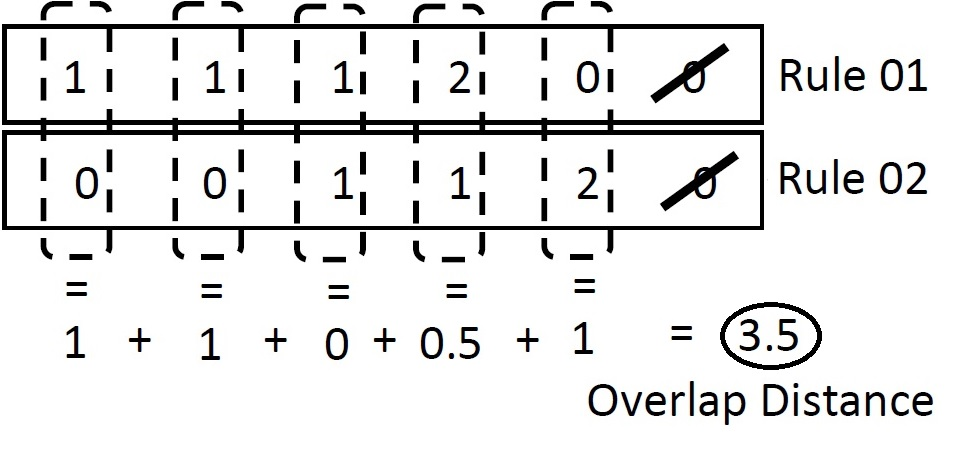
\includegraphics[scale=0.5]{3.jpg}
\end{center}
\label{Fig1}
\caption{Measuring overlap distance}
\end{figure}

\subsection{The Fitness Function}
The main goal of penguins search algorithm is to optimise the
expenditure of energy (run time) and to improve the
quality of generated rules. The generated rules have both
individual and collective quality, the first quality represents
the statistical measure (confidence and support) which is
calculated only from the rule and the transactional database,
whereas, the second one aims to represent the correlation between
the rules (overlap) which is well explained in the previous
section. In the fitness computing, we focused on the first aspect
by taking the rules which maximise the average of the support (Supp) and the confidence (Conf). The fitness value is computed only for the rules satisfying the maximum overlap where
the maximum Overlap (Max-Overlap) is a predefined value that represents the
maximum accepted distance between each pair of rules.
More formally, the fitness function $F$ for a given solution $S$
can be formulated as:\\
\begin{equation}
\label{equa:eq1} F_{max}(S)=\alpha Supp(S) + \beta Conf
(S)
\end{equation}
where $\alpha$ and $\beta$ are two empirical parameters chosen between
$0$ and $1$ and $T$ is the transactional database and \\
\begin{equation*}
Supp(S)= \frac{|\{t \in T | S[i] \neq 0 \Rightarrow S[i]
\subseteq t,  \forall i \in [1..n]\}|}{|T|}
\end{equation*}
\begin{equation*}
Conf(S)= \frac{|\{t \in T | S[i]\neq 0 \Rightarrow
S[i]\subseteq t, \forall i \in [1..n]\}|}{|\{t \in T | S[i]=1
\Rightarrow S[i]\subseteq t, \forall i \in [1..n]\|}\\
\end{equation*}
\\
\textbf{Example:}
\begin{table}[h]
\centering
\begin{tabular}{c c c c}
\hline
$t_{1}$& A & B & C\\
\hline
$t_{2}$& A & B & \\
\hline
$t_{3}$& C & D & \\
\hline
$t_{4}$& E & D & \\
\hline
$t_{5}$& C & A &\\
\hline
\end{tabular}
\caption{Illustration of transactional database for fitness computing}
\label{TransacionalDatabaseIllustration}
\end{table}

Let us consider the transactional database (see
Table~\ref{TransacionalDatabaseIllustration}) that contains $5$
transactions T=$\left\{t_{1}, t_{2}, t_{3}, t_{4}, t_{5}\right\}$ and
$5$ items I=$\left\{A, B, C, D, E \right\}$. For instance, to compute the support
and the confidence of the solution $S=(1,2,0,0,0)$ equivalent to the
rule ($A \rightarrow B$), the number of occurrences of the itemset
(A) and the item set (A,B) should be first determined. We notice that
(A) is repeated $3$ times and (A,B) are repeated together $2$ times.
As a result, the support of (A) is $3/5$ and the support of
(A,B) is $2/5$. So, the confidence of ($A \rightarrow B$) is
$\frac{2/5}{3/5}$ that equals to $2/3$. Now, if we consider
$\alpha=0.5$ and $\beta=0.5$, the fitness of $S$ is :
$F_{max}(S)$ =  ${\left(\frac{1}{2} \times \frac{2}{5}\right)} + {\left(\frac{1}{2} \times
\frac{2}{3}\right)}$, which equal to $\frac{8}{15}$.

\subsection{Algorithm of Pe-ARM}
Pe-ARM algorithm (see Fig.~\ref{algo}) starts with generating a random population of penguins (each penguin represent a rule), this population is divided into groups, each group contains a variable number of penguins which is updated according to the penguins' health. The division of the initial population is based on the amount of overlapping between population rules. 
First a random penguin ($P_{r}$) is selected (center of the first group), and all penguins that have a distance (amount of overlapping) from $P_{r}$ inferior than the min-distance are added to this group. The min-distance is equal to the average of distances between any two rules in the whole population. A new group is created if all other remaining penguins have a distance  from $P_{r}$ superior than the min-distance.
A diversification generation strategy is used to generate K diversified groups in the initial penguin population. Pe-ARM starts with a population distributed in K groups, and each group is placed in a separate region with a minimum distance to any other. The purpose is to start the search with a set of diversified initial solutions which have contrasting features benefiting future solution improvement and to control the non visited region in the coming iterations. Our main goal is to generate a set of consistent rules that have a good fitness with small amount of overlapping between them. The objective function of a given solution $F(P_{i})$ is to maximise the average of statistical measure (confidence and support).
 
Each penguin generates from it's rule another set of rules (neighbours). The best rule among these rules that optimises the objective function is selected. The penguin can move to another position and generate these neighbours  if and only if its oxygen reserve \textbf{$O_{i}$} is not depleted. This oxygen reserve is updated according to the objective function, it represents the health of the penguin. After each iteration, the fitness of the solution of the previous iteration is subtracted from the fitness of the new solution to obtain the value of the oxygen reserve. If the value of the subtraction is positive, the oxygen reserve is incremented to allow this penguin to move to other positions in the next iteration otherwise the oxygen reserve is decremented. The oxygen reserve controls the energy of the penguins in the whole search process. If the oxygen reserve is depleted (equal to zero) the penguins move to another location, either in an existing group or to a new unexplored area. 

All generated rules are firstly validated with the overlap measure $\mu(P_{i})$ before it is evaluated by the objective function. Any solution is validated (passed to the objective function evaluation) if it guarantee the minimum amount of overlap allowed with other accepted rules. The objective function evaluation is performed only for the valid rules because it is usually a high time consuming task for any meta-heuristics based algorithms.

The number of neighbours changes from one penguin to another and it is updated according to the penguin's health (penguin's oxygen reserve). In each iteration, if the oxygen reserve is incremented the number of neighbours is also incremented, in the other case the number of neighbours is decremented. The number of neighbours is initialised to '1', with such situation the penguin can generate only one new position by swapping between the possible values (0,1,2) for one item set. The amount of oxygen allows the penguins to decide to search or not in a given area and the number of neighbours allows penguins to decide to evaluate only a new position or a set of new positions. 

 After each iteration, the penguins communicate with each other the best rule,  $GLbest$, founded  to converge to the best group, update the oxygen reserve and the number of neighbours  for each penguin. The computation of the health of each group is made to  define the probabilities of improvement in each group, and finally we redistribute the penguins on the new population according the health of the penguins of each group (probabilities). 
\begin{figure*}[htbp]
\begin{center}
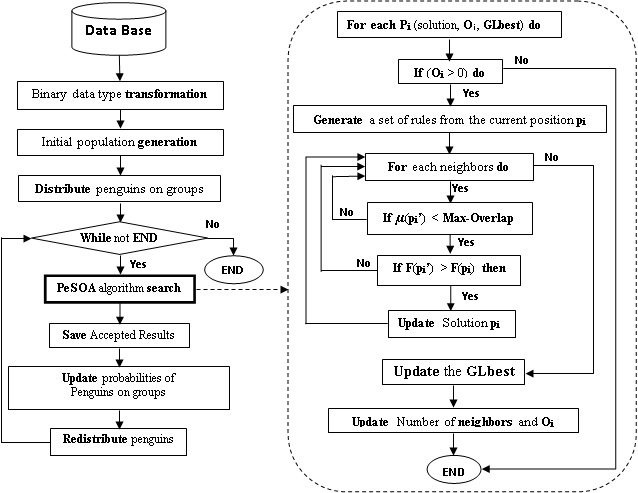
\includegraphics[width=15cm]{2.jpg}
\end{center}
\caption{Penguins Search Optimisation Algorithm For Arm}
\label{algo}
\end{figure*}
\section{Experiments and Results}
In order to evaluate the effectiveness of the proposed algorithm, several evaluation criteria were used in the experimentation process.
Firstly, the statistical measure is computed which is represented as the average of the confidence and the support of the generated rules. 
Secondly, the execution time of each approach is determined. \\
The last measure is the coverage formula which represents the similarities 
between the generated rules according to the number of common transactions. Indeed, 
the rules are similar when they verify together many transactions and dissimilar where
they do not verify any transaction \cite{27}. The coverage formula is given as follows:\\
Let $T_{r_i}$ be the set of transactions verified by $r_{i}$, and $n$ is the number of generated rules.\\
\begin{displaymath}
Coverage =   \frac{\sum_{i=1}^{n}{\sum_{j=1}^{n} {\eta{(r_{i},r_{j})}}}}{n~(n-1)} \\
\end{displaymath}
\begin{displaymath}
\eta{(r_{i},r_{j})} =
\left\lbrace
\begin{array}{ccc}
0          &  i = j & \\
\left|T_{r_{i}} \cup T_{r_{j}}\right| - \left|T_{r_{i}} \cap T_{r_{j}}\right|  & \mbox{Otherwise}  
\end{array}\right.
\end{displaymath}

\subsection{Parameters Settings}
The Penguin search algorithm needs many parameters to ensure the diversification and the intensification properties of the search
process. The aim of this experiment is to find the best parameters to maximise the ratio 
between the average of the fitness of generated rules and the CPU run time. 
In each iteration, we change the parameters in order to find the best stabilised average values. As seen in table 2, when a fewer number of penguins are used the CPU run time is lower, consequently, 
a small part of the rules space is explored, this reduces the quality of the generated rules. In contrast, when the number of penguins 
increases, we get a set of good rules but with increased CPU run time (a 100 generation is used for all tests).

For the number of iterations (table 3), we aim to stabilise the average between the fitness of the solutions and the execution time. It is evident from the table that the fewer the number of iterations the smaller the average of confidence and support and the smaller the execution time. This due to the fact that with a fewer number of iterations a fewer number of rules are generated. However, if the number of iteration is increased the average of confidence and support also increased but with a longer execution time. According to the obtained results, 
the number of iterations is set to $100$ and the number of penguins is set to $25$.
\begin{landscape}
%\clearpage
\begin{table*}[b]
\renewcommand{\arraystretch}{1.3}
\caption{The performance of the PeSOA number of iterations with CPU execution time for different data sets.}
\label{sample-table}
\begin{tabular}{c c c c c c c c c c c c c c c c c c c}
\toprule
\textbf{Data sets} &  \multicolumn{2}{c}{Bolts} & \multicolumn{2}{c}{Sleep} & \multicolumn{2}{c}{Pollution}& \multicolumn{2}{c}{Basket-Ball}& \multicolumn{2}{c}{IBM-Quest}& \multicolumn{2}{c}{Quack}& \multicolumn{2}{c}{Chess}& \multicolumn{2}{c}{Mushroom}\\\midrule
{N Penguins}   & \textbf{F}  & \textbf{t}  & \textbf{F}  & \textbf{t} & \textbf{F}  & \textbf{t} & \textbf{F}  & \textbf{t} & \textbf{F}  & \textbf{t} & \textbf{F}  & \textbf{t} & \textbf{F}  & \textbf{t} & \textbf{F}  & \textbf{t} \\\hline                      
10		&		0.81 & 	0.03		& 		0.88 & 	0.24	&		0.79 & 0.21	&		0.91 & 	0.14		&	 0.81 &	0.19	& 0.81 &  0.54 &	0.80 &	0.61  &	0.78 & 	1.21 \\\hline
15		&		0.85 & 	0.05		& 		0.93 & 	0.31	&		0.91 & 0.28	&		0.95 & 	0.20		&	 0.86 & 0.21	& 0.89 &  0.61 &	0.83 &	0.70  &	0.79 &	1.41 \\\hline
20    &		0.98 & 	0.08		& 		0.97 & 	0.39	&		0.97 & 0.35	&		0.98 & 	0.29		&	 0.90 &	0.25	& 0.90 &  0.69 &	0.87 &	0.76  &	0.81 &  1.58	 \\\hline
25		&		0.99 & 	0.10		& 		0.99 & 	0.46	&		1    & 0.37	&	  0.99 & 	0.31	  &	 0.92 &	0.28	& 0.90 &  0.76 &	0.88 &  0.80  &	0.84 & 	1.67 \\\hline
30		&	  1    & 	0.13		& 		0.99 & 	0.52  &		1    & 0.44	&		0.99 & 	0.37		&	 0.92 &	0.35	& 0.90 &  0.82 &	0.88 &  0.87  &	0.84 &  1.72 \\\hline
35	  &		1    & 	0.18	  & 		0.99 & 	0.57	&		1    & 0.49	&		0.99 & 	0.44 	  &	 0.92 &	0.39	& 0.89 &  0.87 &	0.88 &  0.93  & 0.84 & 	1.79 \\\hline
40	  &		1    & 	0.21		& 		0.97 & 	0.62  &		1    & 0.56	&		0.98 & 	0.46		&	 0.91 &	0.42  & 0.90 &  0.93 &	0.87 &	0.99  &	0.84 & 	1.83 \\\hline
50		&		0.99 & 	0.25	  & 		0.99 & 	0.75	&		1    & 0.62	& 	0.98 & 	0.53		&	 0.92 &	0.56  & 0.90 &  1.10 &	0.88 &	1.15  &	0.82 & 	1.99 \\\hline
60		&		1    & 	0.30		& 		0.98 & 	0.82  &		1    & 0.81	&		0.99 & 	0.61		&	 0.92 &	0.63  & 0.90 &  1.25 &	0.88 &	1.32  &	0.84 & 	2.18 \\\hline
75		&		1    & 	0.41		& 		0.99 & 	0.91	&		1    & 0.95	&		0.99 & 	0.82		&	 0.92 &	0.75  & 0.90 &  1.39 &	0.88 &	1.49 &	0.84 & 	2.32 \\\hline
100		&		1    &  0.62		& 	  0.99 & 	1.14  &		1    & 1.24	&		0.99 & 	1.02		&	 0.92&	0.92  & 0.90 &  1.52 &  0.88 &	1.81 &	0.84 & 	2.61 \\\hline
\bottomrule
\end{tabular}
\end{table*}

\end{landscape}
\begin{landscape}

\begin{table*}[b]
\renewcommand{\arraystretch}{1.3}
\small
\caption{The performance of the PeSOA number of penguins with CPU execution time for different data sets.}
\label{sample-table1}
\begin{tabular}{c c c  c c c c c c c c c c c c c c c c}
\toprule
\textbf{Data sets} &  \multicolumn{2}{c}{Bolts} & \multicolumn{2}{c}{Sleep} & \multicolumn{2}{c}{Pollution}& \multicolumn{2}{c}{Basket-Ball}& \multicolumn{2}{c}{IBM-Quest}& \multicolumn{2}{c}{Quack}& \multicolumn{2}{c}{Chess}& \multicolumn{2}{c}{Mushroom}\\
\midrule
{N Iteration}   & \textbf{F}  & \textbf{t}  & \textbf{F}  & \textbf{t} & \textbf{F}  & \textbf{t} & \textbf{F}  & \textbf{t} & \textbf{F}  & \textbf{t} & \textbf{F}  & \textbf{t} & \textbf{F}  & \textbf{t} & \textbf{F}  & \textbf{t} \\\hline
50		&	  0.94 & 0.04 &	0.81 & 0.21		&		0.91 & 	0.19 	&		0.89 & 0.17	  	&	 0.79 &	0.15	&  0.82 & 0.44  &	0.75 &	0.52  &	0.77 & 	0.85 \\\hline
75		&		0.98 & 0.07 &	0.92 & 0.29 	&		0.95 & 	0.25 	&		0.92 & 0.21	  	&	 0.85 & 0.19	&  0.88 & 0.54  &	0.80 &	0.61  &	0.79 &	1.19  \\\hline
100		&		1    & 0.11	&	0.98 & 0.41 	&		0.99 & 	0.28	&		0.96 & 0.26			&	 0.89 &	0.23	&  0.91 & 0.69  &	0.82 &	0.68  &	0.85 &	1.44   \\\hline
125		&		1    & 0.13	&	0.99 & 0.45 	&		1    & 	0.34	&		0.99 & 0.30			&	 0.92 &	0.27  &  0.90 & 0.75  &	0.88 &  0.77  &	0.84 & 	1.59  \\\hline
150		&	  1    & 0.15	&	1    & 0.48 	&		1    & 	0.37	&		1    & 0.32			&	 0.91 &	0.30  &  0.90 & 0.81  &	0.89 &  0.82  &	0.88 & 	1.64 \\\hline
175		&		1    & 0.18	&	1    & 0.50	  &		1    & 	0.41	&		1    & 0.36		  &	 0.92 &	0.32  &  0.91 & 0.92  &	0.89 &  0.88  & 0.87& 	1.71 \\\hline
200		&		1    & 2.1	&	1    & 0.56 	&		0.99 & 	0.43	&		0.99 & 0.39			&	 0.92 &	0.36  &  0.91 & 1.05  &	0.88 &	0.95  &	0.88 & 	1.79 \\\hline
225		&		1    & 2.5  &	1    & 0.57 	&		0.99 & 	0.46	&		1    & 0.44	  	&	 0.91 &	0.38  &  0.92 & 1.17  &	0.89 &	1.00  &	0.85 & 	1.85 \\\hline
250		&		1    & 2.7	&	1    & 0.62 	&		1    & 	0.50	&		1    & 0.49			&	 0.92 &	0.43  &  0.90 & 1.26  &	0.89 &	1.14  &	0.84 & 	1.93 \\\hline
275		&		1    & 3.0	&	1    & 0.64 	&		0.99 & 	0.54	&		1    & 0.51			&	 0.92 &	0.45  &  0.91 & 1.32  &	0.87 &	1.21 &	0.86 & 	2.05 \\\hline
300		&		0.99 & 3.3	&	1    & 0.68   &		0.99 & 	0.59	&		1    & 0.53   	&	 0.92 &	0.49  &  0.90 & 1.56  &	0.88 &	1.32 &	0.88 &  2.21\\\hline
325		&		1    & 3.8  & 0.98 & 0.70  	&		1    & 	0.62	&		0.99 & 0.56			&	 0.92 &	0.52  &  0.91 & 1.62  &	0.89 &	1.38 &	0.87 & 	2.33 \\\hline
350		&		1    & 4.2	& 0.99 & 0.71		&		0.98 &  0.66	&		1    & 0.59			&	 0.92 &	0.53  &  0.91 & 1.75  &	0.89 &	1.42 &	0.88 & 	2.43 \\\hline
375		&		1    & 4.5  & 1    & 0.73		&		1    & 	0.68	&		0.99 & 0.63			&	 0.91 &	0.54  &  0.91 & 1.86  &	0.88 &	1.49 &	0.89 & 	2.49 \\\hline
400		&		0.99 & 4.7  & 1    & 0.72		&		1    & 	0.73	&		0.99 & 0.67	  	&	 0.92 &	0.61  &  0.92 & 1.96  &	0.89 &	1.55 &	0.87 & 	2.58 \\\hline
425		&		1    & 5.1  & 1    & 0.77		&		1    & 	0.75	&		1    & 0.69			&	 0.91 &	0.63  &  0.90 & 2.10  &	0.78 &	1.61 &	0.87 & 	2.63 \\\hline
450		&		1    & 5.5  & 0.99 & 0.79		&		1    & 	0.78	&		1    & 0.73			&	 0.92 &	0.65  &  0.92 & 2.23  &	0.89 &	1.64 &	0.88 & 	2.71 \\\hline
475		&		1    & 5.4  & 1    & 0.81		&		1    & 	0.82	&		1    & 0.75			&	 0.92 &	0.69  &  0.91 & 2.32  &	0.88 &	1.70 &	0.87 & 	2.88 \\\hline
\bottomrule
\end{tabular}
\end{table*}
\end{landscape}

\subsection{Evaluation with standard data sets}
The following datasets were prepared by \cite{28} from the UCI datasets and PUMSB, 
though they have been converted to Apriori binary format. It has been widely used in 
the evaluation and comparison process for association rule mining problem. These data sets can be classified into three categories-- 
small, medium and large \cite{29}. Table 4 describes the size of the used datasets, the number of transactions and the number
of items in each of the transactions. During performing experiments on standard datasets, the values 0.25, 0.30, 0.75 were used as the minimum support, the minimum confidence and the maximum overlap accepted respectively.
 
\begin{table}[htbp]
\small
\label{datas}
\caption{Standard data sets description}
\begin{center}
\begin{tabular}{c c c}
\toprule
$\textbf{Dataset}$&$\textbf{Transactions size}$&$\textbf{Items size}$\\\hline
\textbf{Bolts}	&40	&8\\\hline
\textbf{Sleep}	&56	&8\\\hline
\textbf{Pollution}	&60	&16\\\hline
\textbf{Basket-Ball}	&96	&5	\\\hline
\textbf{IBM-Quest}	&1000	&40	\\\hline
\textbf{Quack}	&2178	&4	\\\hline
\textbf{Chess}	&3196	&75	\\\hline
\textbf{Mushroom}	&8124	&119 	\\\hline
\bottomrule
\end{tabular}
\end{center}
\end{table}

\begin{table*}[htbp]
\small
\centering
\label{Fig3}
\caption{Comparison of Pe-ARM with different approaches for confidence and support average }
\begin{tabular}{c c c c c c c}
\toprule
\textbf{Data sets} &  Pe-ARM& BSO-ARM & $ACO_{R}$ & SA & G3APARM & ARMBGSA\\
\midrule
\textbf{Bolts}&		1&		1& 0.69 & 0.60 & 0.92 & 0.45\\\hline
\textbf{Sleep}&		1&		1& 0.67 & 0.53 & 0.90 & 0.39\\\hline
\textbf{Pollution}&		1&		1 & 0.66 & 0.50 & 0.92 & 0.56\\\hline
\textbf{Basket-Ball}&	 1&		1 & 0.61 & 0.66 & 0.93 & 0.45\\\hline
\textbf{IBM-Quest}&	 0.92&	0.89 &  0.45 & 0.30 & 0.88 & 0.40\\\hline
\textbf{Quack}&		0.91&		0.89& 0.73 & 0.52 & 0.90 & 0.39\\\hline
\textbf{Chess}&		0.89&		0.86 & 0.3 & 0.15 & 0.86 & 0.38\\\hline
\textbf{Mushroom}&	0.88 &	0.84 & 0.1 & 0.05 & 0.85 &0.35\\\hline
\bottomrule
\end{tabular}
\end{table*}
\begin{table*}[htbp]
\small
\centering
\label{Fig4}
\caption{ Run time (in seconds) comparison among the Pe-ARM and other approaches}
\begin{tabular}{c c c c c c c c c c}
\toprule
\textbf{Data sets} & Pe-ARM& BSO-ARM & $ACO_{R}$ & SA & G3APARM & ARMBGSA \\
\midrule
\textbf{Bolts}&			0.12&		0.22& 1.23 & 1.04 & 0.59 & 1.17 &\\\hline
\textbf{Sleep}&		0.48&		0.95& 2.1 & 2.4 & 0.87 & 1.38 &\\\hline
\textbf{Pollution}&		0.35&		0.62& 1.1 & 1.6 & 0.67 & 1.87 &\\\hline
\textbf{Basket-Ball}&		0.28&		0.56&  1.3 & 1.5 & 0.42 & 2.10 &\\\hline
\textbf{IBM-Quest}&		0.251&	0.32& 0.9 & 1.9 & 0.87 & 1.45 &\\\hline
\textbf{Quack}&		0.67&		0.75&  1.5 & 2.4 & 1.00 & 1.94 &\\\hline
\textbf{Chess}&		0.725&		0.85& 2.4 &  3.02 & 0.99& 2.41 &\\\hline
\textbf{Mushroom}&		1.474&	1.5& 3.6 & 2.8 & 1.84 & 3.98 &\\\hline
\bottomrule
\end{tabular}
\end{table*}
\begin{table*}[htbp]
\small
\centering
\caption{Comparison of Pe-ARM with different approaches for the coverage of 100 generated rules}
\begin{tabular}{c c c c c c c c c c}
\toprule
\textbf{Data sets} & Pe-ARM& BSO-ARM & $ACO_{R}$ & SA & G3APARM & ARMBGSA \\
\midrule
\textbf{Bolts}&11&	7	& 5& 4.12 & 8.24 & 6.25 &\\\hline
\textbf{Sleep}&11.23& 7.5	& 5 & 5.65 & 6.01 & 5.9 &\\\hline
\textbf{Pollution}&11.25&	4.58 & 6.24 & 5.32 & 5.98 & 6.02 &\\\hline
\textbf{Basket-Ball}&12.65&	6.9 & 4.10 & 7.01 & 6.8 & 5 &\\\hline
\textbf{IBM-Quest}&15.2& 6.14	& 6.98 & 4.28 & 6.87 & 7.82 &\\\hline
\textbf{Quack}&21.51&	10.25	& 9.24 & 8.24 & 11.08 & 10.01 &\\\hline
\textbf{Chess}&29.41&	9.27	& 8.21 & 10.36 & 8.52 & 9.88 &\\\hline
\textbf{Mushroom}&35.25& 12.34	& 10.01 & 9.85 & 12.38 & 12.01 &\\\hline
\bottomrule
\end{tabular}
\end{table*}
\newpage
We have compared the performance of Pe-ARM with a set of well known association rule mining algorithms ( BSO-ARM \cite{22} , $ACO_{R}$ \cite{13}, 
SA \cite{30}, G3APARM  \cite{11},  ARMBGSA \cite{21}).
Table 5,6 and 7 summarise all the results obtained by applying Pe-ARM and above mentioned approaches on the various standard datasets. 
The aim is to maximise the average of the statistical measures (confidence and support) and to maximise the overlap 
between rules in order to maximise the coverage.
The proposed Pe-ARM with the new overlap measure gives the best coverage values compare to other  algorithms. This is due to the fact that the set of association rules generated by the Pe-ARM (with the overlap measure) have low overlap between them. 
The mechanism of the penguins algorithm ensures a good intensification  on the way to ameliorate the execution time.

 
\subsection{ Evaluation with Biological data sets}
One of the useful applications of association rules mining is bio-informatics \cite{31}. 
In this section we have used several biological datasets for gene expression under a (sub)set of 
conditions \cite{32,29}. In the context of market basket analysis, gene expression data can be used as a single transaction, 
and each condition as an item.  Also each condition can be validated or not in a given transaction (gene expression).  
Since the gene expression data belong to continuous real values, a discretisation  preprocessing for the gene expression data is needed \cite{33}.
 Datasets values are discretised into two values, 0 if the condition are less-than or equal 0; and 1 otherwise. Table 8 presents the description of the gene expression datasets. During performing experiments on biological datasets, the values 0.20, 0.30, and 0.50 were used as the minimum support, the minimum confidence and the maximum overlap accepted respectively. These values are not fixed, the users are given the flexibility to insert their own values according to the application area.
 
 \begin{table*}
\small
\caption{Biological data sets description}
\begin{center}
\begin{tabular}{c c c}
\toprule
$\textbf{Dataset}$&$\textbf{Transactions size}$&$\textbf{Items size}$\\\hline
\textbf{Leukemia}&	12457&	72 \\\hline
\textbf{Arabidopsis Thaliana}&	73&	69\\\hline
\textbf{Saccharomyces Cerevisiae}&	190&	170\\\hline
\textbf{Yeast}&	94&	174\\\hline
\textbf{Alpha Factor}&	911&	17\\\hline
\textbf{Cdc15}&	607&	607\\\hline
\textbf{Elutriation}&	5632&	15\\\hline
\bottomrule
\end{tabular}
\end{center}
\end{table*}
\begin{table*}[htbp]
\small
\centering
\label{Fig6}
\caption{Comparison of Pe-ARM different approaches with confidence and support average }
\begin{tabular}{c c c c c c c}
\toprule
\textbf{Data sets} &  Pe-ARM& BSO-ARM & $ACO_{R}$ & SA & G3APARM & ARMBGSA\\
\toprule
\textbf{Leukemia}                &	0.78 &	0.68& 0.45 & 0.41	& 0.65 & 0.51	\\\hline
\textbf{Arabidopsis }  &  \multirow{2}{*}{0.64} &  \multirow{2}{*}{0.51}& \multirow{2}{*}{0.41} & \multirow{2}{*}{0.48} & \multirow{2}{*}{0.54} & \multirow{2}{*}{0.39} \\
\textbf{Thaliana} &   & &	 &  &  & \\\hline
\textbf{Saccharomyces}& \multirow{2}{*}{ 0.59 }& \multirow{2}{*}{ 0.38}&	\multirow{2}{*}{0.34} & \multirow{2}{*}{0.31} & \multirow{2}{*}{0.37} & \multirow{2}{*}{0.35}	\\
\textbf{Cerevisiae} &   & &	 &  &  & \\\hline
\textbf{Yeast}                   &	0.55 &	0.38& 0.37 & 0.37 & 0.40 & 0.41 \\\hline
\textbf{Alpha factor}            &	0.64 &	0.46&	0.43 & 0.39	& 0.44 & 0.50	\\\hline
\textbf{Cdc15}                   &	0.62 &	0.43& 0.43 & 0.48 & 0.43 & 0.39	\\\hline
\textbf{Elutriation}             &	0.69 &	0.43&	0.50 & 0.40 & 0.41 & 0.38	\\\hline
\bottomrule
\end{tabular}
\end{table*}
\begin{table*}[htbp]
\small
\centering
\caption{Comparison of Pe-ARM to different approaches with the run time (second)}
\begin{tabular}{c c c c c c c}
\toprule
\textbf{Data sets} & Pe-ARM& BSO-ARM & $ACO_{R}$ & SA & G3APARM & ARMBGSA \\
\midrule
\textbf{Leukemia}                &1.8  &2.4  & 3.8  & 3.1 & 2.61 & 3.01\\\hline
\textbf{Arabidopsis}  & \multirow{2}{*}{0.867}& \multirow{2}{*}{1.875}&  \multirow{2}{*}{2.1}  &  \multirow{2}{*}{1.9} &  \multirow{2}{*}{1.12} &  \multirow{2}{*}{2.10}\\
\textbf{Thaliana} &   & &	 &  &  & \\\hline
\textbf{Saccharomyces}&\multirow{2}{*}{1.283}&\multirow{2}{*}{3.025}&\multirow{2}{*}{ 3.85} & \multirow{2}{*}{2.08}&\multirow{2}{*}{ 2.02} &\multirow{2}{*}{ 1.54}\\
\textbf{Cerevisiae} &   & &	 &  &  & \\\hline
\textbf{Yeast}                   &0.571&1.457& 1.98 & 0.86& 1.42 & 1.04\\\hline
\textbf{Alpha factor}            &0.822&1.958& 2.35 & 2.87& 2.01 & 0.99\\\hline
\textbf{Cdc15}                   &0.704&2.656& 2.99 & 1.05& 2.31 & 1.11\\\hline
\textbf{Elutriation}             &1.339&2.38 & 3.01 & 2.81& 2.15 & 2.51\\\hline
\bottomrule
\end{tabular}
\end{table*}
\begin{table*}
\small
\centering
\caption{Comparison of Pe-ARM to  different approaches with the coverage of 100 rules}
\begin{tabular}{c c c c c c c}
\toprule
\textbf{Data sets} & Pe-ARM& BSO-ARM & $ACO_{R}$ & SA & G3APARM & ARMBGSA \\
\midrule
\textbf{Leukemia}                 &  1273.82  & 645.56 & 512.01 & 496.58 & 715.54 & 544.60 \\\hline
\textbf{Arabidopsis }     &  \multirow{2}{*}{18.46 }     & \multirow{2}{*}{7.45} & \multirow{2}{*}{5.14  } & \multirow{2}{*}{5.27} & \multirow{2}{*}{7.14 }  & \multirow{2}{*}{4.98}  \\
\textbf{Thaliana} &   & &	 &  &  & \\\hline
\textbf{Saccharomyces } &  \multirow{2}{*}{1269.02}  & \multirow{2}{*}{925.46} & \multirow{2}{*}{536.27} & \multirow{2}{*}{821.14} & \multirow{2}{*}{898.74} & \multirow{2}{*}{768.24}  \\
\textbf{Cerevisiae} &   & &	 &  &  & \\\hline

\textbf{Yeast}                    &  224.19    & 100.04& 84.21  & 124.25 & 124.25 & 88.00 \\\hline
\textbf{Alpha factor}             &  461.41   & 221.15 & 102.46 & 98.57 & 184.54 & 113.56\\\hline
\textbf{Cdc15}                    &  620.62    & 252.98&  232.97& 201.62 & 412.32 & 199.85 \\\hline
\textbf{Elutriation}              &  1545.62   & 915.75&  814.65& 901.54 & 754.62 & 865.25\\\hline

\bottomrule
\end{tabular}
\end{table*}


The main motivation behind using biological datasets for evaluation is the 
specificity of gene expression datasets that contains comprehensive and integrated biological information, 
enabling the discovery of functional relationships between those information. Tables 9 shows that the maximum confidence and support for the rules are obtained by using the proposed approach. Interestingly, although the Pe-ARM provides maximum average confidence and support but it takes the minimum amount of run time with compared to other approaches (see Table 10). It is evident from Table 11 that the Pe-ARM provides maximum coverage among all other approaches. It is also seen that the coverage of the final set of association rules for the dataset Elutriation 
is very high as well as the average confidence and support. This can be interpreted as: the set of generated rules are diverse and cover maximum number of different transactions. This is very important for biological datasets because they can grow very large and consist of small items therefore require more coverage. From the results shown in table 9, 10, and 11 we can conclude that the Pe-ARM approach outperforms all other approaches in all regards (e.g. execution time, coverage etc.).
%The confidence and support average of the Pe-ARM has been ameliorated since the use of the Pe-ARM.


%In experimentation of biological data sets cases we have used 0.20, 0.30, 0.50 for minimum support, minimum confidence and minimum overlap accepted, respectively during performing experiments on standard datasets.  

%% \begin{theorem}[ ] ...  \end{theorem}
%% \begin{definition}[ ] ...  \end{definition}
%% \begin{axiom}[ ] ...  \end{axiom}
%% \begin{conjecture}[ ] ...  \end{conjecture}
%% \begin{proposition}[ ] ...  \end{proposition}
%% \begin{corollary}[ ] ...  \end{corollary}
%% \begin{lemma}[ ] ...  \end{lemma}
%% \begin{problem}[ ] ...  \end{problem}
%% \begin{example}[ ] ...  \end{example}
%% \begin{remark}[ ] ...  \end{remark}
%% \begin{proof} ...  \end{proof}
%%
 \section{Conclusion}
In this work a new association rules mining algorithm based on penguins search optimisation 
algorithm (Pe-ARM) has been proposed. To evaluate the amount of overlapping between generated rules, a new way of overlapping measure is incorporated into the main method of the Pe-ARM.  This incorporation helps to generate a set of consistent rules. 
Pe-ARM has been compared with a set of well known meta-heuristics based methods for association rule mining. The comparison was made to evaluate the performance of different methods in terms of computational time, the statistical measure (confidence and support) and finally the coverage measure. Two different types of datasets, e.g., standard and biological, were used to help the evaluation process. The use of biological data sets allows us to validate the approach with data that contain a huge number of association between item sets. The gene expression datasets are made to facilitate different functionalities like extracting rules between conditions of genes. The experiments confirm that the proposed Pe-ARM outperforms all other approaches in terms of statistical measure, coverage, and execution time for both standard and biological datasets. 
Currently, we are investigating to develop a new method to represent large data to further improve the execution time.

%\subsubsection{Caption of the Subsubsection} %Subsubsection


%%%%%%%%%%%%%%%%%%%%%%%%%%%%% Main Text End %%%%%%%%%%%%%%%%%%%%%%%%%%%%%%%%%

\section*{References}
\bibliography{mybibfile}

%\subsubsection{Caption of the Subsubsection} %Subsubsection


%%%%%%%%%%%%%%%%%%%%%%%%%%%%% Main Text End %%%%%%%%%%%%%%%%%%%%%%%%%%%%%%%%%

\end{document}
\endinput
%%
%% End of file `elsarticle-template-num.tex'.
